\documentclass{article}
\newcommand{\templatepath}{../../LaTeX/ubo-template/}
\usepackage{\templatepath ubo}
\usepackage[spanish]{babel}
\usepackage{graphicx}
\usepackage{subcaption}
\usepackage{tocloft}
\setlength{\cftbeforesecskip}{0.5em}
\setlength{\cftbeforesubsecskip}{0.2em}
\renewcommand{\cftsecfont}{\bfseries}
\renewcommand{\cftsubsecfont}{\itshape}
\renewcommand{\cftdot}{·}
\renewcommand{\cftsecleader}{\cftdotfill{\cftdotsep}}
\renewcommand{\cftsecpagefont}{\bfseries}
\usepackage{hyperref}
\hypersetup{
	colorlinks=true,
	linkcolor=black,
	urlcolor=blue,
	citecolor=black,
	bookmarks=true,
	bookmarksopen=true,
	bookmarksnumbered=true,
	pdftitle={Limpieza del dataset Spotify 2023 mediante un pipeline},
	pdfauthor={Aldo Hernández}
}

\begin{document}
	% Portada
	\MakeHeader{Análisis de Datos}{Grupo: TEO 1}{Profesor Eliecer Peña Ancavil}{Limpieza del dataset \textit{Spotify 2023} mediante un \textit{pipeline}}{14 de septiembre de 2025}
	\vfill
	\AuthorRowOne{\CustomAuthor{Aldo Hernández}{haldo@pregrado.ubo.cl}{Universidad Autónoma de Nuevo León}{San Nicolás de los Garza, Nuevo León, MX}}
	\newpage
	
	% Índice
	\tableofcontents
	\listoffigures
	\listoftables
	\thispagestyle{empty}
	\newpage
	
	% Contenido
	\section{Resumen}
	En este informe se busca limpiar el conjunto de datos \textit{Spotify 2023} adaptando un flujo de trabajo utilizado anteriormente a fin de dejarlo listo para un futuro análisis o entrenamiento. Para lograr esto se tuvo que hacer tratamiento de valores nulos mediante imputación y análisis previo de datos atípicos, además de una transformación de valores categóricos a numéricos usando los criterios de \textit{One-Hot Encoding} y \textit{Label Encoding}. Finalmente, logramos reducir el ruido en el dataset y sacar algunas conclusiones previas a un análisis más detallado a pesar de la falta de información en el conjunto de datos. Podemos concluir que la limpieza de datos es un proceso lento pero de vital importancia para un buen análisis de información y buen entrenamiento de modelos, además de que el uso de un flujo de trabajo existente favorece el desarrollo rápido y correcto de este proceso.
	
	\section{Introducción}
	El análisis de datos es una pieza fundamental para el tratamiento de información útil y dar a conocer información oculta en los datos. En este documento aplicaremos el proceso de limpieza de datos para el dataset \textit{Spotify 2023} a fin de dejarlo listo para su posterior análisis o incluso entrenamiento de algún modelo de \textit{Machine Learning}.
	
	Antes de hacer cualquier procedimiento, es fundamental hacer una exploración inicial del dataset que vamos a utilizar para detectar si está listo para usar o no. Es por esto que se definió un flujo de trabajo para la limpieza general de datasets según el conjunto con el que se trabaja, ya que no hay un procedimiento específico que se aplique a todos los conjuntos de datos, sino que se adapta según la información que se maneja.
	
	\subsection{Descripción del problema}
	En este documento, se documentará la limpieza del dataset \textit{Spotify 2023} según un \textit{pipeline} general, adaptándolo según su naturaleza a fin de dejarlo listo para su posterior análisis.
	
	\subsection{Objetivos}
	Este documento busca lo siguiente:
	\begin{itemize}
		\item Reusar un \textit{pipeline} utilizado previamente para otro conjunto de datos y adaptarlo según las circunstancias.
		\item Usar la imputación de valores nulos según la naturaleza de la información.
		\item Limpiar el dataset \textit{Spotify 2023} para prepararlo para su posterior análisis.
	\end{itemize}
	
	\section{Metodología}
	\subsection{Descripción del \textit{dataset}}
	El conjunto de datos contiene información acerca de 952 canciones a lo largo de 10 columnas, sus variables más importantes son:
	\begin{itemize}
		\item track\_name: El nombre de la canción.
		\item in\_spotify\_playlists: La cantidad de playlists en las que fue agregada la canción.
		\item streams: La cantidad de reproducciones.
		\item key: la nota principal de la canción.
		\item mode: la escala de la canción.
		\item danceability\_\%: qué tan "danzable" es la canción.
		\item energy\%: qué tan energética es la canción.
	\end{itemize}
	Este dataset abarca un dominio distinto al de Malenia, acercándonos a la música en lugar de al videojuego \textit{Elden Ring}.
	
	\subsection{Herramientas utilizadas}
	Para la detección de valores atípicos se utilizó el rango intercuartílico y los \textit{boxplots}, para la codificación de variables categóricas se utilizaron dos métodos: el \textit{One-Hot Encoding} y el \textit{Label Encoding}.
	
	Además, se usaron histogramas para la visualización de los datos antes y después de hacer cambios; así como la media, mediana y moda para la imputación de valores nulos.
	
	Por otro lado, en cuanto a codificación se usaron librerías que facilitan el tratamiento de conjuntos grandes de datos y números como \textit{Pandas} y \textit{NumPy}, y otras para la visualización de la información como \textit{Seaborn}.
	
	\section{Análisis de Datos}
	Primero, se hizo una \textbf{exploración inicial} de los datos en la que conocimos la cantidad de registros y columnas, y algunos datos importantes sobre las columnas numéricas como la media aritmética, la desviación estándar y el rango de valores como se observa en la tabla \ref{tab:pre-imp}.
	
	\begin{table}[ht]
		\centering
		\begin{tabular}{lrrrrrrr}
			\hline
			& Año & Mes & Día & Playlists & Reproducciones & Dance\% & Energy\% \\
			\hline
			conteo & 952 & 952 & 952 & 905 & 952 & 905 & 952 \\
			media & 2018 & 6 & 14 & 5273 & 514137400 & 67 & 64 \\
			desv. est. & 11 & 4 & 9 & 7991 & 566856900 & 15 & 17 \\
			min & 1930 & 1 & 1 & 31 & 2762 & 23 & 9 \\
			25\% & 2020 & 3 & 6 & 870 & 141636200 & 57 & 53 \\
			50\% & 2022 & 6 & 13 & 2224 & 290530900 & 69 & 66 \\
			75\% & 2022 & 9 & 22 & 5730 & 673869000 & 78 & 77 \\
			max & 2023 & 12 & 31 & 52898 & 3703895000 & 96 & 97 \\
			\hline
		\end{tabular}
		\caption{Resumen estadístico pre-imputación.}
		\label{tab:pre-imp}
	\end{table}
	
	Luego, se realizó la \textbf{limpieza de los datos} en la que detectamos y tratamos registros sin valores en alguna columna: para las variables categóricas se uso la moda, mientras que para los valores numéricos se decidió usar la mediana en \textit{in\_spotify\_playlists} y la media en \textit{danceability\_\%} debido a la cantidad de registros sin valor que tenían, obteniendo como resultado los cambios definidos en la tabla \ref{tab:post-imp}.
	
	\begin{table}[ht]
		\centering
		\begin{tabular}{lrrrrrrr}
			\hline
			& Año & Mes & Día & Playlists & Reproducciones & Dance\% & Energy\% \\
			\hline
			conteo & 952 & 952 & 952 & 952 & 952 & 952 & 952 \\
			media & 2018 & 6 & 14 & 5123 & 514137400 & 67 & 64 \\
			desv. est. & 11 & 4 & 9 & 7819 & 566856900 & 14 & 17 \\
			min & 1930 & 1 & 1 & 31 & 2762 & 23 & 9 \\
			25\% & 2020 & 3 & 6 & 894 & 141636200 & 58 & 53 \\
			50\% & 2022 & 6 & 13 & 2224 & 290530900 & 68 & 66 \\
			75\% & 2022 & 9 & 22 & 5350 & 673869000 & 78 & 77 \\
			max & 2023 & 12 & 31 & 52898 & 3703895000 & 96 & 97 \\
			\hline
		\end{tabular}
		\caption{Resumen estadístico post-imputación.}
		\label{tab:post-imp}
	\end{table}
	
	Visualmente se puede observar el cambio en la distribución en la columna \textit{danceability\_\%} en la figura \ref{fig:dance_post}. Específicamente para esta columna se utilizó la media para el reemplazo debido a que no tenía tantos valores atípicos, por lo que la distribución se concentró un poco más alrededor de dicho valor.
	
	\newpage
	\begin{figure}[h!] 
		\centering
		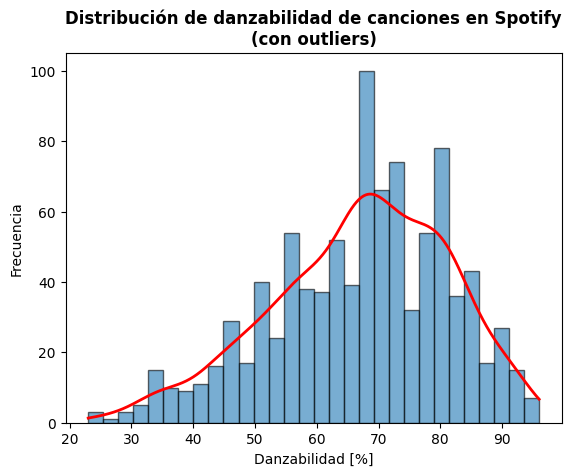
\includegraphics[width=0.5\textwidth]{./danceability_after.png}
		\caption{Distribución final de danceability\%.}
		\label{fig:dance_post}
	\end{figure}
	
	Después, se realizó un análisis para los valores atípicos en el cuál se evaluó si sería mejor reemplazarlos por la media, por la mediana o dejarlos sin cambio alguno. Para elegir una opción fue de mucha ayuda la utilización de gráficos de caja y los histogramas.
	
	\begin{figure}[h!]
		\centering
		\begin{subfigure}[b]{0.45\linewidth}
			\centering
			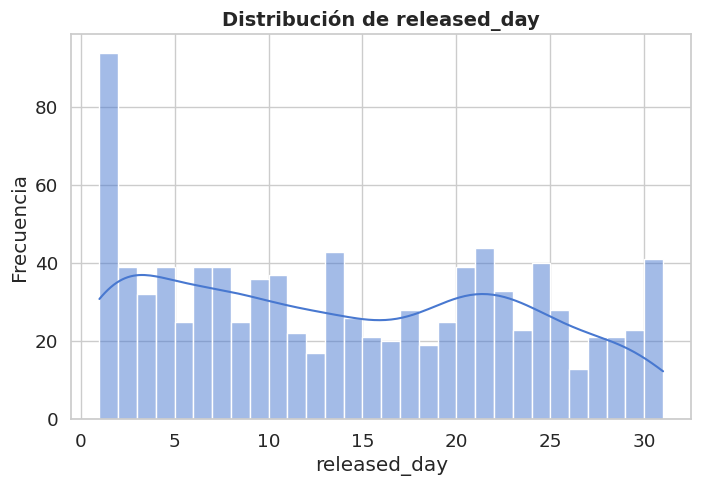
\includegraphics[width=\linewidth]{./day_hist.png}
			\caption{Distribución de días de lanzamiento.}
		\end{subfigure}
		\hfill
		\begin{subfigure}[b]{0.45\linewidth}
			\centering
			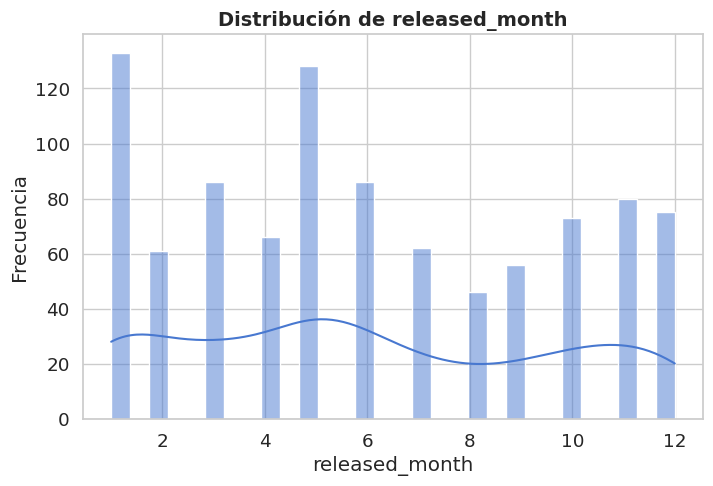
\includegraphics[width=\linewidth]{./month_hist.png}
			\caption{Distribución de meses de lanzamiento.}
		\end{subfigure}
		\hfill
		\begin{subfigure}[b]{0.5\linewidth}
			\centering
			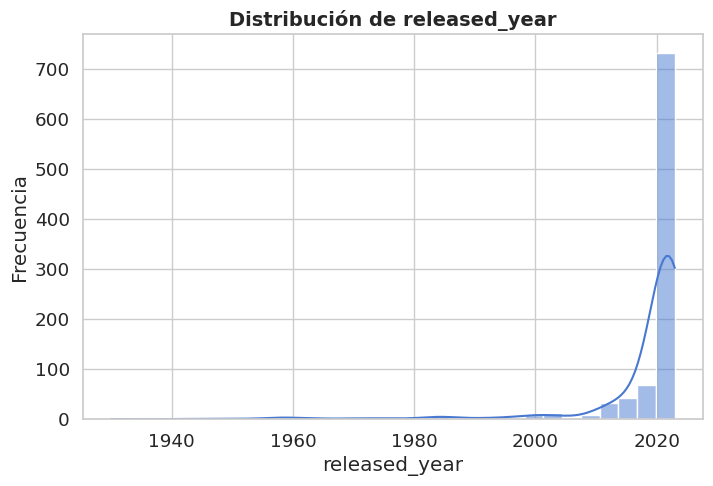
\includegraphics[width=\linewidth]{./year_hist.png}
			\caption{Distribución de años de lanzamiento.}
		\end{subfigure}
		
		\caption{Histogramas de fechas de lanzamiento.}
		\label{fig:fechas_hist}
	\end{figure}
	
	\newpage
	Por ejemplo, de la figura \ref{fig:fechas_hist} podemos concluir que se suelen lanzar más canciones en los primeros días del mes, en enero o mayo y después del 2020.
	
	Por otro lado, en las figuras \ref{fig:pre-streams} y \ref{fig:post-streams} se observa la distribución de los valores antes y después del reemplazo de outliers, en donde se concentran más los datos hacia el valor central.
	
	\begin{figure}[h!]
		\centering
		\begin{subfigure}[b]{0.45\linewidth}
			\centering
			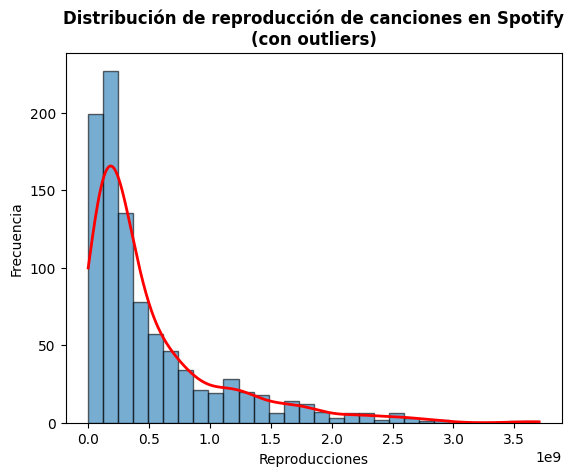
\includegraphics[width=\linewidth]{./streams_before.png}
			\caption{Distribución inicial de streams.}
			\label{fig:pre-streams}
		\end{subfigure}
		\hfill
		\begin{subfigure}[b]{0.45\linewidth}
			\centering
			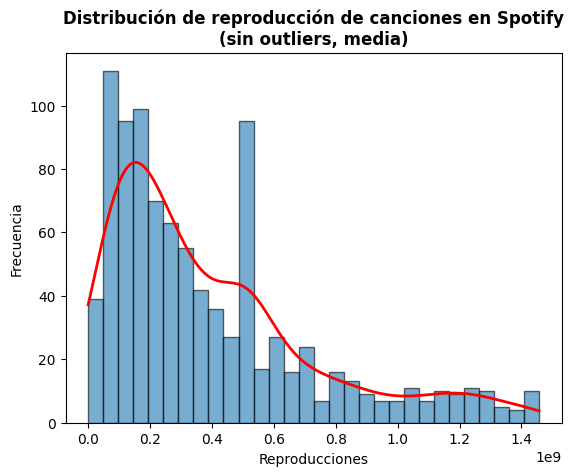
\includegraphics[width=\linewidth]{./streams_after.png}
			\caption{Distribución final de streams.}
			\label{fig:post-streams}
		\end{subfigure}
		\hfill
		
		\caption{Distribución de streams.}
		\label{fig:streams}
	\end{figure}
	
	Finalmente se decidió \textbf{no} hacer ningún cambio a los valores atípicos, ya que se concluyó que no es necesario al ser datos que fueron medidos correctamente y que aportan más información en su forma original para el \textbf{análisis de información}, aunque esto también dependería del alcance que se quiere tener al utilizar este conjunto de datos.
	
	Por último, se utilizó \textit{One Hot Encoding} para la columna \textit{mode} y \textit{Label Encoding} para \textit{key}. Esto se decidió debido a que \textit{mode} es una variable binaria (solo tiene el valor de \textit{Major} o \textit{Minor}), lo cual es muy conveniente para el criterio \textit{One-Hot}; mientras que \textit{key} sigue una jerarquía en sus notas (de más aguda a más grave, por ejemplo) lo cual favorece el uso de esta técnica.
	
	\section{Discusión}
	\subsection{Interpretación de resultados}
	Posterior a este procedimiento, se logró transformar un conjunto de datos con mucho ruido y valores desconocidos en un dataset listo para analizar. La limpieza de los datos puede ser un procedimiento tedioso pero de él depende mucho del éxito que puede tener el análisis hecho, ya que el tratamiento incorrecto de la información puede alterar las conclusiones a las que se pueden llegar (como una mala elección de muestra, datos mal medidos, registros nulos, entre otros); es por esto que hay que conocer las bases esenciales para lograr una buena preparación de los registros.
	
	\subsection{Limitaciones}
	\label{subsec:limitaciones}
	En este conjunto de datos en particular, pensamos que hay tres principales problemas: falta de datos, sesgos y falta de documentación.
	
	Consideramos que cerca de 900 registros concentrados en 10 columnas es muy poca información para realizar un buen análisis o incluso generar un buen modelo de predicción, ya que hay muchas variables que juegan un rol importante pero no han sido incluidas. Además, debido a la cantidad de valores atípicos, se tiene un sesgo en el promedio de algunas columnas como \textit{streams}, lo cual desfavorece el análisis de la información. Por último, no hay suficiente documentación para el conjunto de datos, por ejemplo para algunas columnas (como \textit{streams} o \textit{key}) se puede inferir fácilmente qué es lo que miden y cómo lo miden, pero para las columnas \textit{danceability\_\%} y \textit{energy\_\%} se sabe lo que miden pero no se puede tener ni la más mínima idea de cómo es que se mide dicho valor que incluso se podría argumentar que es subjetivo en ambos casos. Esto ocasiona diversos problemas como la falta de comprensión de la información que se está analizando e incluso la incorrecta creación de columnas (por ejemplo, podría ser mejor dividir la columna \textit{danceability\_\%} en los diversos criterios que conforman dicho valor).
	
	Por otra parte, es probable que la imputación de valores nulos introduzca un sesgo en el conjunto de datos, ya que se trata de cantidades relativamente grandes, por lo que hay que tener cuidado al analizar posteriormente estos datos.
	
	\subsection{Posibles mejoras}
	Aparte de lo mencionado en la subsección \ref{subsec:limitaciones}, el análisis se podría mejorar según el alcance que se quiera tener con él, por ejemplo tal vez sería más beneficioso usar otro método de imputación.
	
	Además, se lograría un mejor análisis de la información si se lograra combinar estos registros con otro conjunto de datos que aporte más información valiosa que sea de nuetro interés, como podría ser la cantidad de artistas participantes o el género musical de la canción.
	
	\section{Conclusiones}
	En este documento se explica todo el proceso de limpieza de datos para su posterior análisis. Según la columna, se utilizó la moda, mediana o moda para imputar los valores nulos; mientras que los valores atípicos no sufrieron ningún cambio debido al valor informativo que aportan.
	
	La implementación de un flujo de trabajo ya existente favoreció el rápido desarrollo del código ya que reducía el trabajo a solamente adaptar los bloques de código según la naturaleza del conjunto de datos.
	
	Además, podemos determinar algunas observaciones interesantes, como que los artistas suelen lanzar música en los primeros días del mes y más comúnmente en enero o mayo.
	
	Por otro lado, la falta de información es un factor que afecta gravemente el valor de análisis de este conjunto de datos, por lo que si no se maneja con cuidado se pueden conseguir conclusiones imprecisas o erróneas, o incluso introducir sesgos en la información.
	
	Por último, es importante mencionar que todo análisis carece de valor si no es intepretado correctamente, por lo que hay que conocer a detalle el alcance que se quiere tener con el dataset antes de analizarlo para definir un proceso de limpieza específico acorde a la finalidad del estudio. Este tipo de procesos son de vital importancia para la toma de decisiones en el mundo real mediante análisis estadístico puro o implementación de modelos de \textit{machine learning} e incrementar su eficacia.
	
	\section{Bibliografía}
	No se utilizó ninguna fuente de información externa para el desarrollo de este informe. El notebook se puede encontrar en la siguiente \hyperlink{https://colab.research.google.com/drive/1gEqeVx9LOfKF7kmSRVEvj6D3_2fIOvWQ?usp=sharing}{\underline{liga}}.
\end{document}